\documentclass{standalone}
\usepackage{pgfplots}
\pgfplotsset{
  compat=1.18, 
  ticklabel style = {font=\footnotesize},
  axis equal image,
}

\begin{document}
  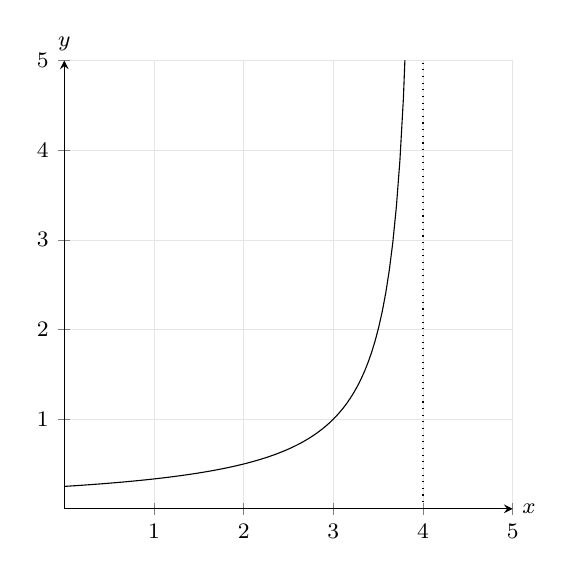
\begin{tikzpicture}
    \begin{axis}[
      axis lines=middle,
      xmin=0, xmax=5,
      ymin=0, ymax=5,
      xlabel={\footnotesize \(x\)},
      xlabel style={at={(ticklabel* cs:1)}, anchor=west},
      ylabel={\footnotesize \(y\)},
      ylabel style={at={(ticklabel* cs:1)}, anchor=south},
      axis line style = {thin},
      grid=both,
      grid style={line width=.2pt, draw=gray!20},
      ]
      \addplot[no marks, samples=100, domain=0:3.9] { 1/(4 - x) };
      \addplot[dotted] coordinates { (4,0) (4,10) };
    \end{axis}
  \end{tikzpicture}
\end{document}

